%%%%%%%%%%%%%%%%%%%%%%%%
%
% $Autor: Hemanth Jadiswami Prabhakaran $
% $Datum: 2026-09-12 $
% $Pfad: GitHub/MBIDA_Thesis/report/Contents/General/en/07DevelopmentToDeployment.tex $
% $Version: 1 $
%
% $Project: MBIDA Thesis $
%
%%%%%%%%%%%%%%%%%%%%%%%%

\chapter{Development to Deployment}
\label{chap:devToDeployment}

This chapter turns from the model fitting and reconciliation implementation described in Chapter~\ref{chap:appDevelopment} to how that implementation is organised as a codebase: the single configuration module shared by both notebooks and the dashboard (Section~\ref{sec:configPy}), what is required to reproduce the reported results exactly (Section~\ref{sec:reproducibility}), and the layout of the repository that holds all of this together (Section~\ref{sec:repoLayout}). The dashboard that consumes the artifacts this codebase produces is presented in Chapter~\ref{chap:appDeployment}.

\section{\texttt{Code/config.py} as the Single Source of Truth}
\label{sec:configPy}

Three separate entry points read from the same underlying definitions: the exploratory notebook, the forecasting pipeline, and the deployed dashboard. \texttt{01\_eda.ipynb} and \texttt{02\_pipeline.ipynb} both live in \texttt{Code/notebooks/} and import \texttt{Code/config.py} by appending its parent directory to \texttt{sys.path} before importing it as \texttt{cfg}; \texttt{app/streamlit\_app.py} does the same, appending its own parent's parent directory so the import resolves regardless of the working directory the app is launched from -- a detail that matters because Streamlit Community Cloud always sets the working directory to the repository root, not to \texttt{app/}. Figure~\ref{fig:configPyHub} shows the resulting relationship: \texttt{config.py} sits at the centre, and all three consumers read from it rather than from one another.

\begin{figure}[H]
	\centering
	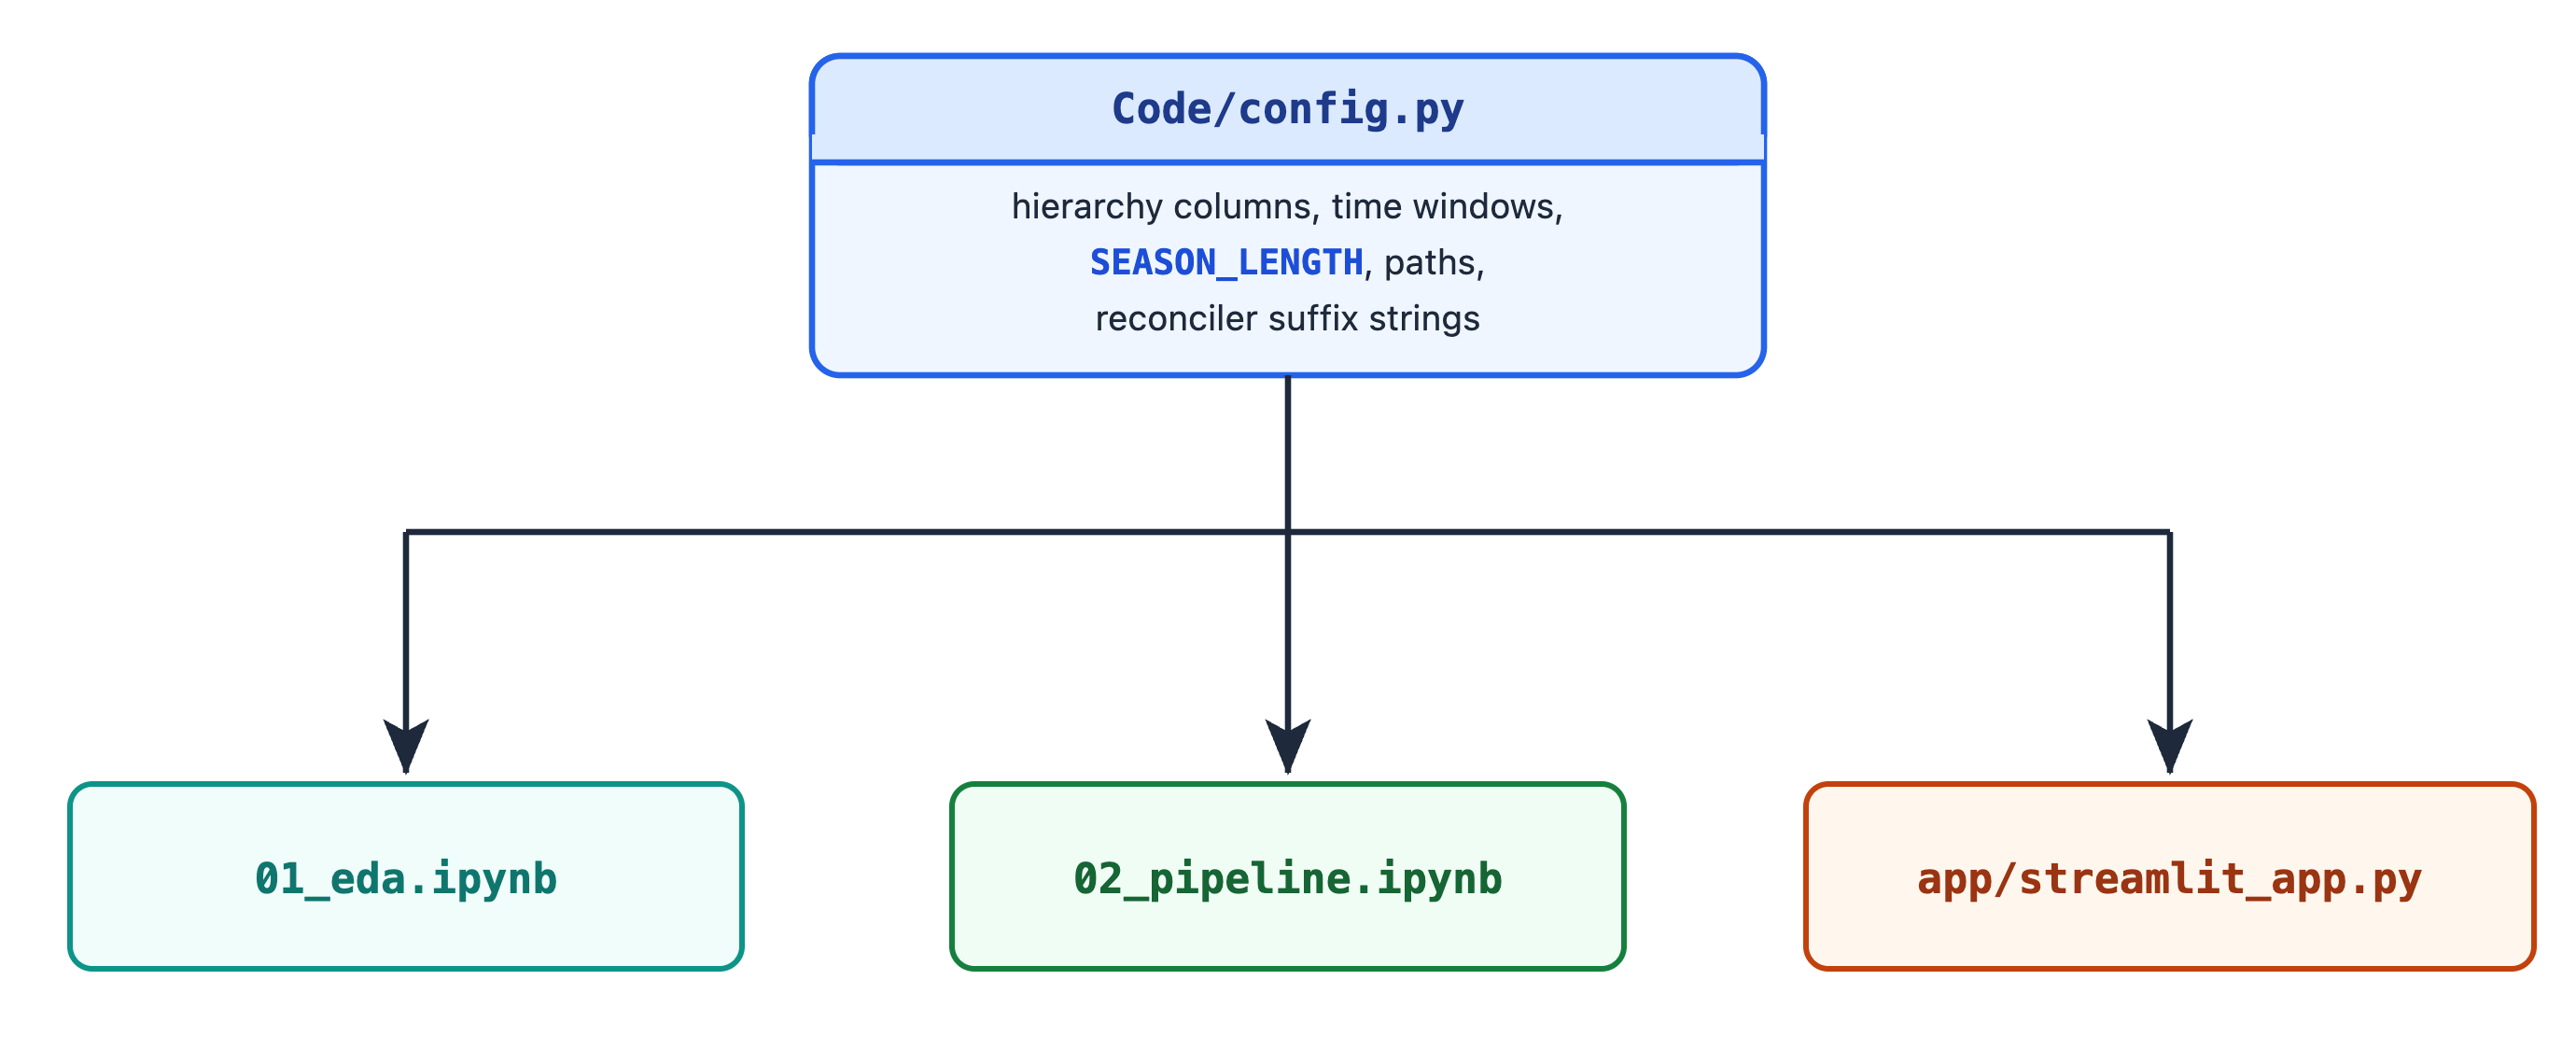
\includegraphics[width=1\linewidth]{Images/07DevelopmentToDeployment/configPyHub}
	\caption{\texttt{Code/config.py} as the single configuration module feeding both notebooks and the Streamlit app.}\label{fig:configPyHub}
\end{figure}




\texttt{config.py} centralises everything that would otherwise have to be kept in sync by hand across these three files: the column names used throughout (\texttt{DATE\_COL}, \texttt{TARGET\_COL}, \texttt{ID\_COL}, \texttt{CAT\_LABEL\_COL}), the six hierarchy columns from \texttt{COL\_TOTAL} down to \texttt{COL\_ITEM} together with the \texttt{SPEC} list that \texttt{hierarchicalforecast}'s \texttt{aggregate()} function uses to build the hierarchy, the three time-window boundaries (\texttt{TRAIN\_TEST\_SPLIT\_DATE}, \texttt{FORECAST\_START\_DATE}, \texttt{FORECAST\_END\_DATE}), the seasonal period \texttt{SEASON\_LENGTH}, the volume-bucket \texttt{PERCENTILES}, the data and cache directory paths, and the mapping from each reconciler to the column-suffix it produces (e.g. \texttt{BottomUpSparse}, \texttt{MinTraceSparse\_method-wls\_struct\_nonnegative-True}). A representative import looks the same wherever it appears:

\begin{Python}
	import sys
	from pathlib import Path
	sys.path.append(str(Path("..").resolve()))
	import config as cfg
\end{Python}

The value of this is that the dashboard's own hierarchy-navigation logic -- which builds node labels by joining the same column names with \texttt{config.LEVEL\_SEP} -- and the pipeline's aggregation step both read the same \texttt{SPEC} and the same column constants, so a change to the hierarchy definition (adding a level, renaming a column) only has to be made once, in one file, rather than tracked down separately in a notebook and an app. This is the "Don't Repeat Yourself" (DRY) principle applied to configuration rather than to code: every piece of shared knowledge has a single, authoritative representation, so no other file can silently drift out of sync with it \cite{Hunt:1999}. \texttt{Code/README.md} documents this convention for anyone extending the codebase.

\section{Reproducibility}
\label{sec:reproducibility}

Every result reported in this thesis was produced by running \texttt{02\_pipeline.ipynb} top-to-bottom, once, in a dedicated \texttt{m5\_forecast} environment, rather than by executing individual cells out of order. This matters beyond general good practice: it is precisely the first of the standard rules for reproducible computational research, keeping track of exactly how every result was produced rather than relying on an undocumented sequence of manual steps \cite{Sandve:2013}. Several steps in the pipeline depend on state built by earlier cells, most notably the item-universe fix, which removes items with no training-period sales before the hierarchy, the base models, and every downstream evaluation are built -- re-running only a later cell after changing an earlier one would silently leave stale, larger item and forecast tables in memory. The documented rule is accordingly to re-run the whole notebook from the top whenever the underlying data, \texttt{config.py}, or any modelling step changes.

Two further conventions support reproducing these results exactly. First, the raw M5 CSV files (\texttt{sales\_train\_validation.csv}, 30,490 rows of one item-store series each, and \texttt{calendar.csv}) are cached to Parquet the first time they are loaded, and every subsequent run reads the cached Parquet file instead of re-parsing the CSV. This is purely a performance measure -- Parquet is a columnar binary format that reads back faster than a CSV and preserves column types, so dates remain dates rather than being re-parsed from strings on every run -- and it has no effect on the values produced, since the cache is a lossless copy of the same CSV. This raw cache lives under \texttt{Code/artifacts/raw\_cache/} and is excluded from version control, since it is fully regenerable from the Kaggle source files. Second, the pipeline environment itself is version-pinned, following the same guidelines' third rule of archiving the exact versions of every external program a result depends on \cite{Sandve:2013}: \texttt{requirements-pipeline.txt} fixes the exact versions of every package the notebooks depend on (for example \texttt{pandas} 2.3.3, \texttt{numpy} 2.2.6, \texttt{statsforecast} 2.1.1, \texttt{hierarchicalforecast} 1.5.1, \texttt{utilsforecast} 0.2.16, and \texttt{pyarrow} 24.0.0), so that re-creating the \texttt{m5\_forecast} environment from this file reproduces the same library behaviour rather than whatever happens to be the current release of each package at some later date.

The four small Parquet files the pipeline exports for the dashboard (Section~\ref{sec:configPy} lists the shared paths that govern where these are written) are treated differently from the raw cache: at a few megabytes each, they are committed to the repository directly, so the deployed dashboard has data to read without needing to re-run the pipeline in the deployment environment at all -- a point taken up in Chapter~\ref{chap:appDeployment}.

\section{Repo Layout and Separation of Concerns}
\label{sec:repoLayout}

The repository is organised so that each of the three consumers described in Section~\ref{sec:configPy} owns only the part of the codebase specific to it, with \texttt{config.py} as the one file all three share:

\begin{itemize}
	\item \texttt{Code/config.py} -- the shared configuration module described above.
	\item \texttt{Code/notebooks/} -- \texttt{01\_eda.ipynb} and \texttt{02\_pipeline.ipynb}, the exploratory analysis and the forecasting pipeline.
	\item \texttt{Code/app/} -- \texttt{streamlit\_app.py} and its own \texttt{requirements.txt}, the minimal package list Streamlit Community Cloud actually installs at deployment time.
	\item \texttt{Code/artifacts/dashboard\_data/} -- the four committed Parquet files the app reads.
	\item \texttt{Code/artifacts/raw\_cache/} -- the gitignored Parquet cache of the raw Kaggle CSVs, described in Section~\ref{sec:reproducibility}.
	\item \texttt{Code/data/} -- a \texttt{README.md} explaining where to place the Kaggle competition files, plus \texttt{Code/data/m5/}, itself gitignored since the competition data cannot be redistributed.
	\item \texttt{Code/requirements-pipeline.txt} -- the pinned local research environment described in Section~\ref{sec:reproducibility}, distinct from \texttt{Code/app/requirements.txt}.
	\item \texttt{.streamlit/config.toml} -- kept at the true repository root rather than nested under \texttt{Code/} or \texttt{Code/app/}, because Streamlit Community Cloud only looks for this file at the root of the deployed repository.
\end{itemize}

The notebooks themselves are kept fully self-contained, with all logic written inline rather than factored out into an importable \texttt{src/} package. Given that the codebase consists of exactly two notebooks feeding one dashboard script, introducing a separate package layer would add a level of indirection without a corresponding benefit; \texttt{config.py} already serves as the only module genuinely shared across more than one file, and nothing else in the pipeline is reused elsewhere. This separation is also what keeps the app itself simple: as its own module docstring states, \texttt{streamlit\_app.py} reads exclusively from the four Parquet files in \texttt{Code/artifacts/dashboard\_data/} and never re-runs the pipeline itself, since Streamlit Community Cloud only ever executes that one file.